
%---------------------------------------------------------------------------------------------------------------------------------------------------%

\noindent \textbf{Types of Channel}
\textbf{ 1. Lossless Channel:}\\
A channel described by a channel matrix with only one non-zero element in each column is called a lossless channel.


\[  [P(Y|X)]  =  \left[ \begin{array}{ccccc}
3/4 & 1/4 &0 & 0&0\\
0  & 0 &1/3 & 2/3& 0\\
0  & 0& 0&0 &1 \\
\end{array} \right]  \]
%(Drawn in overhead):\\ \bigskip

It can be shown that in the lossless channel, no source information is lost in transmission.

%---------------------------------------------------------------------------------------------------------------------------------------------------%

\noindent \textbf{Types of Channel}
\textbf{ 1. Lossless Channel:}\\

\begin{figure}
\centering
\includegraphics[width=0.7\linewidth]{./11Blossless}
\caption{}
\label{fig:11Blossless}
\end{figure}




%---------------------------------------------------------------------------------------------------------------------------------------------------%

\noindent \textbf{Types of Channel}
\textbf{2. Deterministic Channel:}\\
A channel described by a channel matrix with only one non-zero element in each row is called a deterministic channel.

\[  [P(Y|X)]  =  \left[ \begin{array}{ccc}
1   & 0 &0 \\
1  & 0 &0\\
0  & 1 &0\\
0  & 1& 0 \\
0  & 0& 1 \\
\end{array} \right]  \]
%(Drawn in overhead):\\ \bigskip
Note that since each row has only one non-zero element, this element must be 1. When a given source symbol is sent in a deterministic channel, it is clear which output symbol would be received.


%---------------------------------------------------------------------------------------------------------------------------------------------------%

\noindent \textbf{Types of Channel}
\textbf{2. Deterministic Channel:}\\
\begin{figure}
\centering
\includegraphics[width=0.7\linewidth]{./11Bdeterministic}
\caption{}
\label{fig:11Bdeterministic}
\end{figure}



%---------------------------------------------------------------------------------------------------------------------------------------------------%

\noindent \textbf{Types of Channel}
\textbf{3. Noiseless Channel:}\\
A channel is said to be \emph{\textbf{noiseless}} if it is both lossless and deterministic.
The channel matrix is the identity matrix: only one element in each row and each column, and each element is necessarily 1.
\[  [P(Y|X)]  = \left[ \begin{array}{cccc}
1 &0 & \ldots & 0 \\
0 & 1& \ldots & 0 \\
\ldots & \ldots & \ldots & \ldots \\
0& 0 & \ldots & 1 \\
\end{array} \right] \]
%(Drawn in overhead):\\ \bigskip
Note that the input and output alphabets have the same size , i.e. $m=n$.


\noindent \textbf{Types of Channel}
\textbf{3. Noiseless Channel:}\\
\begin{figure}
\centering
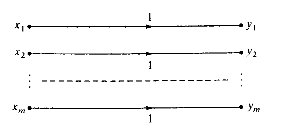
\includegraphics[width=0.7\linewidth]{./11BNoiseless}
\caption{}
\label{fig:11BNoiseless}
\end{figure}


%----------------------------------------------------------------------------------------------------------------------------------------------------%

\noindent \textbf{Types of Channel}
\textbf{4. Binary Symmetric Channel:}\\
The binary symmetric channel is defined by the following channel diagram (next slide) and the channel matrix is given by

\[  [P(Y|X)]  = \left[ \begin{array}{cc}
1-p & p  \\
p & 1-p\\
\end{array} \right] \]
The channel has two inputs and two outputs $(x_1=0,x_2=1)$ and two outputs $(x_1=0,x_2=1)$. The channel is symmetric because the probability of receiving a 1 if a 0 is sent is the same as the probability of receiving a 0 if a 1 was sent. This common probability is denoted $p$.


{
\noindent \textbf{Binary Symmetric Channels}

\begin{center}
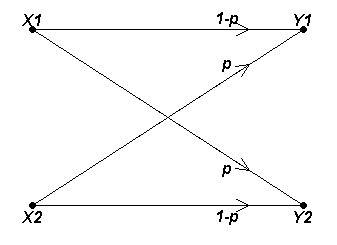
\includegraphics[scale=0.54]{11aBSC}
\end{center}
}

